% Graphic for TeX using PGF
% Title: /home/ameen/Desktop/methodology.dia
% Creator: Dia v0.97.1
% CreationDate: Sat Jan  4 03:50:51 2014
% For: ameen
% \usepackage{tikz}
% The following commands are not supported in PSTricks at present
% We define them conditionally, so when they are implemented,
% this pgf file will use them.
\ifx\du\undefined
  \newlength{\du}
\fi
\setlength{\du}{30\unitlength}
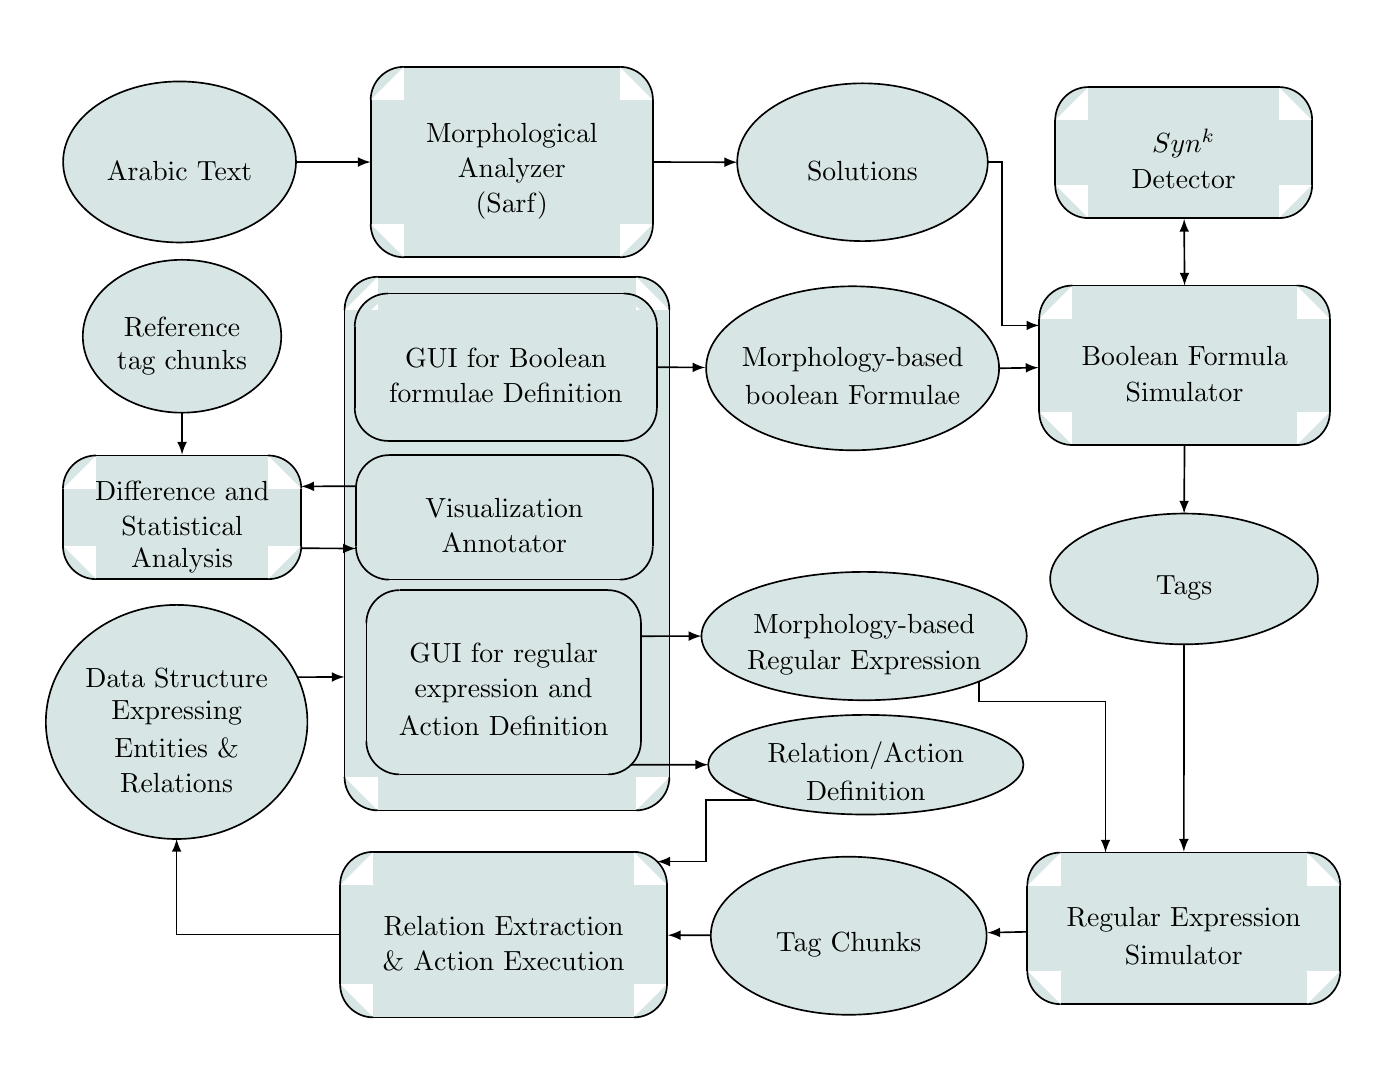
\begin{tikzpicture}
\pgftransformxscale{1.000000}
\pgftransformyscale{-1.000000}
\definecolor{dialinecolor}{rgb}{0.000000, 0.000000, 0.000000}
\pgfsetstrokecolor{dialinecolor}
\definecolor{dialinecolor}{rgb}{1.000000, 1.000000, 1.000000}
\pgfsetfillcolor{dialinecolor}
\definecolor{dialinecolor}{rgb}{0.847059, 0.898039, 0.898039}
\pgfsetfillcolor{dialinecolor}
\pgfpathellipse{\pgfpoint{4.104323\du}{3.277242\du}}{\pgfpoint{1.402453\du}{0\du}}{\pgfpoint{0\du}{0.969732\du}}
\pgfusepath{fill}
\pgfsetlinewidth{0.020000\du}
\pgfsetdash{}{0pt}
\pgfsetdash{}{0pt}
\pgfsetmiterjoin
\definecolor{dialinecolor}{rgb}{0.000000, 0.000000, 0.000000}
\pgfsetstrokecolor{dialinecolor}
\pgfpathellipse{\pgfpoint{4.104323\du}{3.277242\du}}{\pgfpoint{1.402453\du}{0\du}}{\pgfpoint{0\du}{0.969732\du}}
\pgfusepath{stroke}
% setfont left to latex
\definecolor{dialinecolor}{rgb}{0.000000, 0.000000, 0.000000}
\pgfsetstrokecolor{dialinecolor}
\node at (4.104323\du,3.380576\du){Arabic Text};
\definecolor{dialinecolor}{rgb}{0.847059, 0.898039, 0.898039}
\pgfsetfillcolor{dialinecolor}
\fill (6.806370\du,2.131640\du)--(6.806370\du,4.425246\du)--(9.406370\du,4.425246\du)--(9.406370\du,2.131640\du)--cycle;
\definecolor{dialinecolor}{rgb}{0.847059, 0.898039, 0.898039}
\pgfsetfillcolor{dialinecolor}
\pgfpathmoveto{\pgfpoint{6.806381\du}{2.131640\du}}
\pgfpatharc{270}{180}{0.400000\du and 0.400000\du}
\pgfusepath{fill}
\definecolor{dialinecolor}{rgb}{0.847059, 0.898039, 0.898039}
\pgfsetfillcolor{dialinecolor}
\pgfpathmoveto{\pgfpoint{9.806370\du}{2.531640\du}}
\pgfpatharc{360}{270}{0.400000\du and 0.400000\du}
\pgfusepath{fill}
\definecolor{dialinecolor}{rgb}{0.847059, 0.898039, 0.898039}
\pgfsetfillcolor{dialinecolor}
\fill (6.406370\du,2.531640\du)--(6.406370\du,4.025246\du)--(9.806370\du,4.025246\du)--(9.806370\du,2.531640\du)--cycle;
\definecolor{dialinecolor}{rgb}{0.847059, 0.898039, 0.898039}
\pgfsetfillcolor{dialinecolor}
\pgfpathmoveto{\pgfpoint{6.406370\du}{4.025225\du}}
\pgfpatharc{180}{90}{0.400000\du and 0.400000\du}
\pgfusepath{fill}
\definecolor{dialinecolor}{rgb}{0.847059, 0.898039, 0.898039}
\pgfsetfillcolor{dialinecolor}
\pgfpathmoveto{\pgfpoint{9.406338\du}{4.425246\du}}
\pgfpatharc{90}{0}{0.400000\du and 0.400000\du}
\pgfusepath{fill}
\pgfsetlinewidth{0.020000\du}
\pgfsetdash{}{0pt}
\pgfsetdash{}{0pt}
\pgfsetmiterjoin
\definecolor{dialinecolor}{rgb}{0.000000, 0.000000, 0.000000}
\pgfsetstrokecolor{dialinecolor}
\draw (6.806370\du,2.131640\du)--(9.406370\du,2.131640\du);
\definecolor{dialinecolor}{rgb}{0.000000, 0.000000, 0.000000}
\pgfsetstrokecolor{dialinecolor}
\draw (6.806370\du,4.425246\du)--(9.406370\du,4.425246\du);
\definecolor{dialinecolor}{rgb}{0.000000, 0.000000, 0.000000}
\pgfsetstrokecolor{dialinecolor}
\pgfpathmoveto{\pgfpoint{6.806381\du}{2.131640\du}}
\pgfpatharc{270}{180}{0.400000\du and 0.400000\du}
\pgfusepath{stroke}
\definecolor{dialinecolor}{rgb}{0.000000, 0.000000, 0.000000}
\pgfsetstrokecolor{dialinecolor}
\pgfpathmoveto{\pgfpoint{9.806370\du}{2.531640\du}}
\pgfpatharc{360}{270}{0.400000\du and 0.400000\du}
\pgfusepath{stroke}
\definecolor{dialinecolor}{rgb}{0.000000, 0.000000, 0.000000}
\pgfsetstrokecolor{dialinecolor}
\draw (6.406370\du,2.531640\du)--(6.406370\du,4.025246\du);
\definecolor{dialinecolor}{rgb}{0.000000, 0.000000, 0.000000}
\pgfsetstrokecolor{dialinecolor}
\draw (9.806370\du,2.531640\du)--(9.806370\du,4.025246\du);
\definecolor{dialinecolor}{rgb}{0.000000, 0.000000, 0.000000}
\pgfsetstrokecolor{dialinecolor}
\pgfpathmoveto{\pgfpoint{6.406370\du}{4.025225\du}}
\pgfpatharc{180}{90}{0.400000\du and 0.400000\du}
\pgfusepath{stroke}
\definecolor{dialinecolor}{rgb}{0.000000, 0.000000, 0.000000}
\pgfsetstrokecolor{dialinecolor}
\pgfpathmoveto{\pgfpoint{9.406338\du}{4.425246\du}}
\pgfpatharc{90}{0}{0.400000\du and 0.400000\du}
\pgfusepath{stroke}
% setfont left to latex
\definecolor{dialinecolor}{rgb}{0.000000, 0.000000, 0.000000}
\pgfsetstrokecolor{dialinecolor}
\node at (8.106370\du,2.958443\du){Morphological};
% setfont left to latex
\definecolor{dialinecolor}{rgb}{0.000000, 0.000000, 0.000000}
\pgfsetstrokecolor{dialinecolor}
\node at (8.106370\du,3.381776\du){Analyzer};
% setfont left to latex
\definecolor{dialinecolor}{rgb}{0.000000, 0.000000, 0.000000}
\pgfsetstrokecolor{dialinecolor}
\node at (8.106370\du,3.805110\du){(Sarf)};
\definecolor{dialinecolor}{rgb}{0.847059, 0.898039, 0.898039}
\pgfsetfillcolor{dialinecolor}
\pgfpathellipse{\pgfpoint{12.330127\du}{3.280471\du}}{\pgfpoint{1.508827\du}{0\du}}{\pgfpoint{0\du}{0.950191\du}}
\pgfusepath{fill}
\pgfsetlinewidth{0.020000\du}
\pgfsetdash{}{0pt}
\pgfsetdash{}{0pt}
\pgfsetmiterjoin
\definecolor{dialinecolor}{rgb}{0.000000, 0.000000, 0.000000}
\pgfsetstrokecolor{dialinecolor}
\pgfpathellipse{\pgfpoint{12.330127\du}{3.280471\du}}{\pgfpoint{1.508827\du}{0\du}}{\pgfpoint{0\du}{0.950191\du}}
\pgfusepath{stroke}
% setfont left to latex
\definecolor{dialinecolor}{rgb}{0.000000, 0.000000, 0.000000}
\pgfsetstrokecolor{dialinecolor}
\node at (12.330127\du,3.383804\du){Solutions};
\definecolor{dialinecolor}{rgb}{0.847059, 0.898039, 0.898039}
\pgfsetfillcolor{dialinecolor}
\fill (14.859100\du,4.765980\du)--(14.859100\du,6.687033\du)--(17.560450\du,6.687033\du)--(17.560450\du,4.765980\du)--cycle;
\definecolor{dialinecolor}{rgb}{0.847059, 0.898039, 0.898039}
\pgfsetfillcolor{dialinecolor}
\pgfpathmoveto{\pgfpoint{14.859111\du}{4.765980\du}}
\pgfpatharc{270}{180}{0.400000\du and 0.400000\du}
\pgfusepath{fill}
\definecolor{dialinecolor}{rgb}{0.847059, 0.898039, 0.898039}
\pgfsetfillcolor{dialinecolor}
\pgfpathmoveto{\pgfpoint{17.960450\du}{5.165980\du}}
\pgfpatharc{360}{270}{0.400000\du and 0.400000\du}
\pgfusepath{fill}
\definecolor{dialinecolor}{rgb}{0.847059, 0.898039, 0.898039}
\pgfsetfillcolor{dialinecolor}
\fill (14.459100\du,5.165980\du)--(14.459100\du,6.287033\du)--(17.960450\du,6.287033\du)--(17.960450\du,5.165980\du)--cycle;
\definecolor{dialinecolor}{rgb}{0.847059, 0.898039, 0.898039}
\pgfsetfillcolor{dialinecolor}
\pgfpathmoveto{\pgfpoint{14.459100\du}{6.287012\du}}
\pgfpatharc{180}{90}{0.400000\du and 0.400000\du}
\pgfusepath{fill}
\definecolor{dialinecolor}{rgb}{0.847059, 0.898039, 0.898039}
\pgfsetfillcolor{dialinecolor}
\pgfpathmoveto{\pgfpoint{17.560418\du}{6.687033\du}}
\pgfpatharc{90}{0}{0.400000\du and 0.400000\du}
\pgfusepath{fill}
\pgfsetlinewidth{0.020000\du}
\pgfsetdash{}{0pt}
\pgfsetdash{}{0pt}
\pgfsetmiterjoin
\definecolor{dialinecolor}{rgb}{0.000000, 0.000000, 0.000000}
\pgfsetstrokecolor{dialinecolor}
\draw (14.859100\du,4.765980\du)--(17.560450\du,4.765980\du);
\definecolor{dialinecolor}{rgb}{0.000000, 0.000000, 0.000000}
\pgfsetstrokecolor{dialinecolor}
\draw (14.859100\du,6.687033\du)--(17.560450\du,6.687033\du);
\definecolor{dialinecolor}{rgb}{0.000000, 0.000000, 0.000000}
\pgfsetstrokecolor{dialinecolor}
\pgfpathmoveto{\pgfpoint{14.859111\du}{4.765980\du}}
\pgfpatharc{270}{180}{0.400000\du and 0.400000\du}
\pgfusepath{stroke}
\definecolor{dialinecolor}{rgb}{0.000000, 0.000000, 0.000000}
\pgfsetstrokecolor{dialinecolor}
\pgfpathmoveto{\pgfpoint{17.960450\du}{5.165980\du}}
\pgfpatharc{360}{270}{0.400000\du and 0.400000\du}
\pgfusepath{stroke}
\definecolor{dialinecolor}{rgb}{0.000000, 0.000000, 0.000000}
\pgfsetstrokecolor{dialinecolor}
\draw (14.459100\du,5.165980\du)--(14.459100\du,6.287033\du);
\definecolor{dialinecolor}{rgb}{0.000000, 0.000000, 0.000000}
\pgfsetstrokecolor{dialinecolor}
\draw (17.960450\du,5.165980\du)--(17.960450\du,6.287033\du);
\definecolor{dialinecolor}{rgb}{0.000000, 0.000000, 0.000000}
\pgfsetstrokecolor{dialinecolor}
\pgfpathmoveto{\pgfpoint{14.459100\du}{6.287012\du}}
\pgfpatharc{180}{90}{0.400000\du and 0.400000\du}
\pgfusepath{stroke}
\definecolor{dialinecolor}{rgb}{0.000000, 0.000000, 0.000000}
\pgfsetstrokecolor{dialinecolor}
\pgfpathmoveto{\pgfpoint{17.560418\du}{6.687033\du}}
\pgfpatharc{90}{0}{0.400000\du and 0.400000\du}
\pgfusepath{stroke}
% setfont left to latex
\definecolor{dialinecolor}{rgb}{0.000000, 0.000000, 0.000000}
\pgfsetstrokecolor{dialinecolor}
\node at (16.209775\du,5.618173\du){Boolean Formula};
% setfont left to latex
\definecolor{dialinecolor}{rgb}{0.000000, 0.000000, 0.000000}
\pgfsetstrokecolor{dialinecolor}
\node at (16.209775\du,6.041506\du){Simulator};
\definecolor{dialinecolor}{rgb}{0.847059, 0.898039, 0.898039}
\pgfsetfillcolor{dialinecolor}
\fill (15.051700\du,2.375000\du)--(15.051700\du,3.953590\du)--(17.346550\du,3.953590\du)--(17.346550\du,2.375000\du)--cycle;
\definecolor{dialinecolor}{rgb}{0.847059, 0.898039, 0.898039}
\pgfsetfillcolor{dialinecolor}
\pgfpathmoveto{\pgfpoint{15.051711\du}{2.375000\du}}
\pgfpatharc{270}{180}{0.400000\du and 0.400000\du}
\pgfusepath{fill}
\definecolor{dialinecolor}{rgb}{0.847059, 0.898039, 0.898039}
\pgfsetfillcolor{dialinecolor}
\pgfpathmoveto{\pgfpoint{17.746550\du}{2.775000\du}}
\pgfpatharc{360}{270}{0.400000\du and 0.400000\du}
\pgfusepath{fill}
\definecolor{dialinecolor}{rgb}{0.847059, 0.898039, 0.898039}
\pgfsetfillcolor{dialinecolor}
\fill (14.651700\du,2.775000\du)--(14.651700\du,3.553590\du)--(17.746550\du,3.553590\du)--(17.746550\du,2.775000\du)--cycle;
\definecolor{dialinecolor}{rgb}{0.847059, 0.898039, 0.898039}
\pgfsetfillcolor{dialinecolor}
\pgfpathmoveto{\pgfpoint{14.651700\du}{3.553569\du}}
\pgfpatharc{180}{90}{0.400000\du and 0.400000\du}
\pgfusepath{fill}
\definecolor{dialinecolor}{rgb}{0.847059, 0.898039, 0.898039}
\pgfsetfillcolor{dialinecolor}
\pgfpathmoveto{\pgfpoint{17.346518\du}{3.953590\du}}
\pgfpatharc{90}{0}{0.400000\du and 0.400000\du}
\pgfusepath{fill}
\pgfsetlinewidth{0.020000\du}
\pgfsetdash{}{0pt}
\pgfsetdash{}{0pt}
\pgfsetmiterjoin
\definecolor{dialinecolor}{rgb}{0.000000, 0.000000, 0.000000}
\pgfsetstrokecolor{dialinecolor}
\draw (15.051700\du,2.375000\du)--(17.346550\du,2.375000\du);
\definecolor{dialinecolor}{rgb}{0.000000, 0.000000, 0.000000}
\pgfsetstrokecolor{dialinecolor}
\draw (15.051700\du,3.953590\du)--(17.346550\du,3.953590\du);
\definecolor{dialinecolor}{rgb}{0.000000, 0.000000, 0.000000}
\pgfsetstrokecolor{dialinecolor}
\pgfpathmoveto{\pgfpoint{15.051711\du}{2.375000\du}}
\pgfpatharc{270}{180}{0.400000\du and 0.400000\du}
\pgfusepath{stroke}
\definecolor{dialinecolor}{rgb}{0.000000, 0.000000, 0.000000}
\pgfsetstrokecolor{dialinecolor}
\pgfpathmoveto{\pgfpoint{17.746550\du}{2.775000\du}}
\pgfpatharc{360}{270}{0.400000\du and 0.400000\du}
\pgfusepath{stroke}
\definecolor{dialinecolor}{rgb}{0.000000, 0.000000, 0.000000}
\pgfsetstrokecolor{dialinecolor}
\draw (14.651700\du,2.775000\du)--(14.651700\du,3.553590\du);
\definecolor{dialinecolor}{rgb}{0.000000, 0.000000, 0.000000}
\pgfsetstrokecolor{dialinecolor}
\draw (17.746550\du,2.775000\du)--(17.746550\du,3.553590\du);
\definecolor{dialinecolor}{rgb}{0.000000, 0.000000, 0.000000}
\pgfsetstrokecolor{dialinecolor}
\pgfpathmoveto{\pgfpoint{14.651700\du}{3.553569\du}}
\pgfpatharc{180}{90}{0.400000\du and 0.400000\du}
\pgfusepath{stroke}
\definecolor{dialinecolor}{rgb}{0.000000, 0.000000, 0.000000}
\pgfsetstrokecolor{dialinecolor}
\pgfpathmoveto{\pgfpoint{17.346518\du}{3.953590\du}}
\pgfpatharc{90}{0}{0.400000\du and 0.400000\du}
\pgfusepath{stroke}
% setfont left to latex
\definecolor{dialinecolor}{rgb}{0.000000, 0.000000, 0.000000}
\pgfsetstrokecolor{dialinecolor}
\node at (16.199125\du,3.055962\du){$Syn^k$};
% setfont left to latex
\definecolor{dialinecolor}{rgb}{0.000000, 0.000000, 0.000000}
\pgfsetstrokecolor{dialinecolor}
\node at (16.199125\du,3.479295\du){Detector};
\definecolor{dialinecolor}{rgb}{0.847059, 0.898039, 0.898039}
\pgfsetfillcolor{dialinecolor}
\pgfpathellipse{\pgfpoint{16.203500\du}{8.299829\du}}{\pgfpoint{1.612500\du}{0\du}}{\pgfpoint{0\du}{0.787489\du}}
\pgfusepath{fill}
\pgfsetlinewidth{0.020000\du}
\pgfsetdash{}{0pt}
\pgfsetdash{}{0pt}
\pgfsetmiterjoin
\definecolor{dialinecolor}{rgb}{0.000000, 0.000000, 0.000000}
\pgfsetstrokecolor{dialinecolor}
\pgfpathellipse{\pgfpoint{16.203500\du}{8.299829\du}}{\pgfpoint{1.612500\du}{0\du}}{\pgfpoint{0\du}{0.787489\du}}
\pgfusepath{stroke}
% setfont left to latex
\definecolor{dialinecolor}{rgb}{0.000000, 0.000000, 0.000000}
\pgfsetstrokecolor{dialinecolor}
\node at (16.203500\du,8.403162\du){Tags};
\definecolor{dialinecolor}{rgb}{0.847059, 0.898039, 0.898039}
\pgfsetfillcolor{dialinecolor}
\fill (14.715400\du,11.595600\du)--(14.715400\du,13.421754\du)--(17.685400\du,13.421754\du)--(17.685400\du,11.595600\du)--cycle;
\definecolor{dialinecolor}{rgb}{0.847059, 0.898039, 0.898039}
\pgfsetfillcolor{dialinecolor}
\pgfpathmoveto{\pgfpoint{14.715411\du}{11.595600\du}}
\pgfpatharc{270}{180}{0.400000\du and 0.400000\du}
\pgfusepath{fill}
\definecolor{dialinecolor}{rgb}{0.847059, 0.898039, 0.898039}
\pgfsetfillcolor{dialinecolor}
\pgfpathmoveto{\pgfpoint{18.085400\du}{11.995600\du}}
\pgfpatharc{360}{270}{0.400000\du and 0.400000\du}
\pgfusepath{fill}
\definecolor{dialinecolor}{rgb}{0.847059, 0.898039, 0.898039}
\pgfsetfillcolor{dialinecolor}
\fill (14.315400\du,11.995600\du)--(14.315400\du,13.021754\du)--(18.085400\du,13.021754\du)--(18.085400\du,11.995600\du)--cycle;
\definecolor{dialinecolor}{rgb}{0.847059, 0.898039, 0.898039}
\pgfsetfillcolor{dialinecolor}
\pgfpathmoveto{\pgfpoint{14.315400\du}{13.021733\du}}
\pgfpatharc{180}{90}{0.400000\du and 0.400000\du}
\pgfusepath{fill}
\definecolor{dialinecolor}{rgb}{0.847059, 0.898039, 0.898039}
\pgfsetfillcolor{dialinecolor}
\pgfpathmoveto{\pgfpoint{17.685368\du}{13.421754\du}}
\pgfpatharc{90}{0}{0.400000\du and 0.400000\du}
\pgfusepath{fill}
\pgfsetlinewidth{0.020000\du}
\pgfsetdash{}{0pt}
\pgfsetdash{}{0pt}
\pgfsetmiterjoin
\definecolor{dialinecolor}{rgb}{0.000000, 0.000000, 0.000000}
\pgfsetstrokecolor{dialinecolor}
\draw (14.715400\du,11.595600\du)--(17.685400\du,11.595600\du);
\definecolor{dialinecolor}{rgb}{0.000000, 0.000000, 0.000000}
\pgfsetstrokecolor{dialinecolor}
\draw (14.715400\du,13.421754\du)--(17.685400\du,13.421754\du);
\definecolor{dialinecolor}{rgb}{0.000000, 0.000000, 0.000000}
\pgfsetstrokecolor{dialinecolor}
\pgfpathmoveto{\pgfpoint{14.715411\du}{11.595600\du}}
\pgfpatharc{270}{180}{0.400000\du and 0.400000\du}
\pgfusepath{stroke}
\definecolor{dialinecolor}{rgb}{0.000000, 0.000000, 0.000000}
\pgfsetstrokecolor{dialinecolor}
\pgfpathmoveto{\pgfpoint{18.085400\du}{11.995600\du}}
\pgfpatharc{360}{270}{0.400000\du and 0.400000\du}
\pgfusepath{stroke}
\definecolor{dialinecolor}{rgb}{0.000000, 0.000000, 0.000000}
\pgfsetstrokecolor{dialinecolor}
\draw (14.315400\du,11.995600\du)--(14.315400\du,13.021754\du);
\definecolor{dialinecolor}{rgb}{0.000000, 0.000000, 0.000000}
\pgfsetstrokecolor{dialinecolor}
\draw (18.085400\du,11.995600\du)--(18.085400\du,13.021754\du);
\definecolor{dialinecolor}{rgb}{0.000000, 0.000000, 0.000000}
\pgfsetstrokecolor{dialinecolor}
\pgfpathmoveto{\pgfpoint{14.315400\du}{13.021733\du}}
\pgfpatharc{180}{90}{0.400000\du and 0.400000\du}
\pgfusepath{stroke}
\definecolor{dialinecolor}{rgb}{0.000000, 0.000000, 0.000000}
\pgfsetstrokecolor{dialinecolor}
\pgfpathmoveto{\pgfpoint{17.685368\du}{13.421754\du}}
\pgfpatharc{90}{0}{0.400000\du and 0.400000\du}
\pgfusepath{stroke}
% setfont left to latex
\definecolor{dialinecolor}{rgb}{0.000000, 0.000000, 0.000000}
\pgfsetstrokecolor{dialinecolor}
\node at (16.200400\du,12.400344\du){Regular Expression};
% setfont left to latex
\definecolor{dialinecolor}{rgb}{0.000000, 0.000000, 0.000000}
\pgfsetstrokecolor{dialinecolor}
\node at (16.200400\du,12.823677\du){Simulator};
\definecolor{dialinecolor}{rgb}{0.847059, 0.898039, 0.898039}
\pgfsetfillcolor{dialinecolor}
\pgfpathellipse{\pgfpoint{12.164219\du}{12.597547\du}}{\pgfpoint{1.661219\du}{0\du}}{\pgfpoint{0\du}{0.951847\du}}
\pgfusepath{fill}
\pgfsetlinewidth{0.020000\du}
\pgfsetdash{}{0pt}
\pgfsetdash{}{0pt}
\pgfsetmiterjoin
\definecolor{dialinecolor}{rgb}{0.000000, 0.000000, 0.000000}
\pgfsetstrokecolor{dialinecolor}
\pgfpathellipse{\pgfpoint{12.164219\du}{12.597547\du}}{\pgfpoint{1.661219\du}{0\du}}{\pgfpoint{0\du}{0.951847\du}}
\pgfusepath{stroke}
% setfont left to latex
\definecolor{dialinecolor}{rgb}{0.000000, 0.000000, 0.000000}
\pgfsetstrokecolor{dialinecolor}
\node at (12.164219\du,12.700880\du){Tag Chunks};
\definecolor{dialinecolor}{rgb}{0.847059, 0.898039, 0.898039}
\pgfsetfillcolor{dialinecolor}
\fill (6.438190\du,11.587300\du)--(6.438190\du,13.580906\du)--(9.575690\du,13.580906\du)--(9.575690\du,11.587300\du)--cycle;
\definecolor{dialinecolor}{rgb}{0.847059, 0.898039, 0.898039}
\pgfsetfillcolor{dialinecolor}
\pgfpathmoveto{\pgfpoint{6.438201\du}{11.587300\du}}
\pgfpatharc{270}{180}{0.400000\du and 0.400000\du}
\pgfusepath{fill}
\definecolor{dialinecolor}{rgb}{0.847059, 0.898039, 0.898039}
\pgfsetfillcolor{dialinecolor}
\pgfpathmoveto{\pgfpoint{9.975690\du}{11.987300\du}}
\pgfpatharc{360}{270}{0.400000\du and 0.400000\du}
\pgfusepath{fill}
\definecolor{dialinecolor}{rgb}{0.847059, 0.898039, 0.898039}
\pgfsetfillcolor{dialinecolor}
\fill (6.038190\du,11.987300\du)--(6.038190\du,13.180906\du)--(9.975690\du,13.180906\du)--(9.975690\du,11.987300\du)--cycle;
\definecolor{dialinecolor}{rgb}{0.847059, 0.898039, 0.898039}
\pgfsetfillcolor{dialinecolor}
\pgfpathmoveto{\pgfpoint{6.038190\du}{13.180885\du}}
\pgfpatharc{180}{90}{0.400000\du and 0.400000\du}
\pgfusepath{fill}
\definecolor{dialinecolor}{rgb}{0.847059, 0.898039, 0.898039}
\pgfsetfillcolor{dialinecolor}
\pgfpathmoveto{\pgfpoint{9.575658\du}{13.580906\du}}
\pgfpatharc{90}{0}{0.400000\du and 0.400000\du}
\pgfusepath{fill}
\pgfsetlinewidth{0.020000\du}
\pgfsetdash{}{0pt}
\pgfsetdash{}{0pt}
\pgfsetmiterjoin
\definecolor{dialinecolor}{rgb}{0.000000, 0.000000, 0.000000}
\pgfsetstrokecolor{dialinecolor}
\draw (6.438190\du,11.587300\du)--(9.575690\du,11.587300\du);
\definecolor{dialinecolor}{rgb}{0.000000, 0.000000, 0.000000}
\pgfsetstrokecolor{dialinecolor}
\draw (6.438190\du,13.580906\du)--(9.575690\du,13.580906\du);
\definecolor{dialinecolor}{rgb}{0.000000, 0.000000, 0.000000}
\pgfsetstrokecolor{dialinecolor}
\pgfpathmoveto{\pgfpoint{6.438201\du}{11.587300\du}}
\pgfpatharc{270}{180}{0.400000\du and 0.400000\du}
\pgfusepath{stroke}
\definecolor{dialinecolor}{rgb}{0.000000, 0.000000, 0.000000}
\pgfsetstrokecolor{dialinecolor}
\pgfpathmoveto{\pgfpoint{9.975690\du}{11.987300\du}}
\pgfpatharc{360}{270}{0.400000\du and 0.400000\du}
\pgfusepath{stroke}
\definecolor{dialinecolor}{rgb}{0.000000, 0.000000, 0.000000}
\pgfsetstrokecolor{dialinecolor}
\draw (6.038190\du,11.987300\du)--(6.038190\du,13.180906\du);
\definecolor{dialinecolor}{rgb}{0.000000, 0.000000, 0.000000}
\pgfsetstrokecolor{dialinecolor}
\draw (9.975690\du,11.987300\du)--(9.975690\du,13.180906\du);
\definecolor{dialinecolor}{rgb}{0.000000, 0.000000, 0.000000}
\pgfsetstrokecolor{dialinecolor}
\pgfpathmoveto{\pgfpoint{6.038190\du}{13.180885\du}}
\pgfpatharc{180}{90}{0.400000\du and 0.400000\du}
\pgfusepath{stroke}
\definecolor{dialinecolor}{rgb}{0.000000, 0.000000, 0.000000}
\pgfsetstrokecolor{dialinecolor}
\pgfpathmoveto{\pgfpoint{9.575658\du}{13.580906\du}}
\pgfpatharc{90}{0}{0.400000\du and 0.400000\du}
\pgfusepath{stroke}
% setfont left to latex
\definecolor{dialinecolor}{rgb}{0.000000, 0.000000, 0.000000}
\pgfsetstrokecolor{dialinecolor}
\node at (8.006940\du,12.475770\du){Relation Extraction};
% setfont left to latex
\definecolor{dialinecolor}{rgb}{0.000000, 0.000000, 0.000000}
\pgfsetstrokecolor{dialinecolor}
\node at (8.006940\du,12.899103\du){\& Action Execution};
\definecolor{dialinecolor}{rgb}{0.847059, 0.898039, 0.898039}
\pgfsetfillcolor{dialinecolor}
\pgfpathellipse{\pgfpoint{4.069199\du}{10.022428\du}}{\pgfpoint{1.575149\du}{0\du}}{\pgfpoint{0\du}{1.409758\du}}
\pgfusepath{fill}
\pgfsetlinewidth{0.020000\du}
\pgfsetdash{}{0pt}
\pgfsetdash{}{0pt}
\pgfsetmiterjoin
\definecolor{dialinecolor}{rgb}{0.000000, 0.000000, 0.000000}
\pgfsetstrokecolor{dialinecolor}
\pgfpathellipse{\pgfpoint{4.069199\du}{10.022428\du}}{\pgfpoint{1.575149\du}{0\du}}{\pgfpoint{0\du}{1.409758\du}}
\pgfusepath{stroke}
% setfont left to latex
\definecolor{dialinecolor}{rgb}{0.000000, 0.000000, 0.000000}
\pgfsetstrokecolor{dialinecolor}
\node at (4.069199\du,9.490761\du){Data Structure};
% setfont left to latex
\definecolor{dialinecolor}{rgb}{0.000000, 0.000000, 0.000000}
\pgfsetstrokecolor{dialinecolor}
\node at (4.069199\du,9.914094\du){Expressing};
% setfont left to latex
\definecolor{dialinecolor}{rgb}{0.000000, 0.000000, 0.000000}
\pgfsetstrokecolor{dialinecolor}
\node at (4.069199\du,10.337428\du){Entities \& };
% setfont left to latex
\definecolor{dialinecolor}{rgb}{0.000000, 0.000000, 0.000000}
\pgfsetstrokecolor{dialinecolor}
\node at (4.069199\du,10.760761\du){Relations};
\definecolor{dialinecolor}{rgb}{0.847059, 0.898039, 0.898039}
\pgfsetfillcolor{dialinecolor}
\fill (3.099980\du,6.812670\du)--(3.099980\du,8.302670\du)--(5.170380\du,8.302670\du)--(5.170380\du,6.812670\du)--cycle;
\definecolor{dialinecolor}{rgb}{0.847059, 0.898039, 0.898039}
\pgfsetfillcolor{dialinecolor}
\pgfpathmoveto{\pgfpoint{3.099991\du}{6.812670\du}}
\pgfpatharc{270}{180}{0.400000\du and 0.400000\du}
\pgfusepath{fill}
\definecolor{dialinecolor}{rgb}{0.847059, 0.898039, 0.898039}
\pgfsetfillcolor{dialinecolor}
\pgfpathmoveto{\pgfpoint{5.570380\du}{7.212670\du}}
\pgfpatharc{360}{270}{0.400000\du and 0.400000\du}
\pgfusepath{fill}
\definecolor{dialinecolor}{rgb}{0.847059, 0.898039, 0.898039}
\pgfsetfillcolor{dialinecolor}
\fill (2.699980\du,7.212670\du)--(2.699980\du,7.902670\du)--(5.570380\du,7.902670\du)--(5.570380\du,7.212670\du)--cycle;
\definecolor{dialinecolor}{rgb}{0.847059, 0.898039, 0.898039}
\pgfsetfillcolor{dialinecolor}
\pgfpathmoveto{\pgfpoint{2.699980\du}{7.902649\du}}
\pgfpatharc{180}{90}{0.400000\du and 0.400000\du}
\pgfusepath{fill}
\definecolor{dialinecolor}{rgb}{0.847059, 0.898039, 0.898039}
\pgfsetfillcolor{dialinecolor}
\pgfpathmoveto{\pgfpoint{5.170349\du}{8.302670\du}}
\pgfpatharc{90}{0}{0.400000\du and 0.400000\du}
\pgfusepath{fill}
\pgfsetlinewidth{0.020000\du}
\pgfsetdash{}{0pt}
\pgfsetdash{}{0pt}
\pgfsetmiterjoin
\definecolor{dialinecolor}{rgb}{0.000000, 0.000000, 0.000000}
\pgfsetstrokecolor{dialinecolor}
\draw (3.099980\du,6.812670\du)--(5.170380\du,6.812670\du);
\definecolor{dialinecolor}{rgb}{0.000000, 0.000000, 0.000000}
\pgfsetstrokecolor{dialinecolor}
\draw (3.099980\du,8.302670\du)--(5.170380\du,8.302670\du);
\definecolor{dialinecolor}{rgb}{0.000000, 0.000000, 0.000000}
\pgfsetstrokecolor{dialinecolor}
\pgfpathmoveto{\pgfpoint{3.099991\du}{6.812670\du}}
\pgfpatharc{270}{180}{0.400000\du and 0.400000\du}
\pgfusepath{stroke}
\definecolor{dialinecolor}{rgb}{0.000000, 0.000000, 0.000000}
\pgfsetstrokecolor{dialinecolor}
\pgfpathmoveto{\pgfpoint{5.570380\du}{7.212670\du}}
\pgfpatharc{360}{270}{0.400000\du and 0.400000\du}
\pgfusepath{stroke}
\definecolor{dialinecolor}{rgb}{0.000000, 0.000000, 0.000000}
\pgfsetstrokecolor{dialinecolor}
\draw (2.699980\du,7.212670\du)--(2.699980\du,7.902670\du);
\definecolor{dialinecolor}{rgb}{0.000000, 0.000000, 0.000000}
\pgfsetstrokecolor{dialinecolor}
\draw (5.570380\du,7.212670\du)--(5.570380\du,7.902670\du);
\definecolor{dialinecolor}{rgb}{0.000000, 0.000000, 0.000000}
\pgfsetstrokecolor{dialinecolor}
\pgfpathmoveto{\pgfpoint{2.699980\du}{7.902649\du}}
\pgfpatharc{180}{90}{0.400000\du and 0.400000\du}
\pgfusepath{stroke}
\definecolor{dialinecolor}{rgb}{0.000000, 0.000000, 0.000000}
\pgfsetstrokecolor{dialinecolor}
\pgfpathmoveto{\pgfpoint{5.170349\du}{8.302670\du}}
\pgfpatharc{90}{0}{0.400000\du and 0.400000\du}
\pgfusepath{stroke}
% setfont left to latex
\definecolor{dialinecolor}{rgb}{0.000000, 0.000000, 0.000000}
\pgfsetstrokecolor{dialinecolor}
\node at (4.135180\du,7.237670\du){Difference and };
% setfont left to latex
\definecolor{dialinecolor}{rgb}{0.000000, 0.000000, 0.000000}
\pgfsetstrokecolor{dialinecolor}
\node at (4.135180\du,7.661003\du){Statistical};
% setfont left to latex
\definecolor{dialinecolor}{rgb}{0.000000, 0.000000, 0.000000}
\pgfsetstrokecolor{dialinecolor}
\node at (4.135180\du,8.084337\du){Analysis};
\pgfsetlinewidth{0.020000\du}
\pgfsetdash{}{0pt}
\pgfsetdash{}{0pt}
\pgfsetbuttcap
{
\definecolor{dialinecolor}{rgb}{0.000000, 0.000000, 0.000000}
\pgfsetfillcolor{dialinecolor}
% was here!!!
\pgfsetarrowsend{latex}
\definecolor{dialinecolor}{rgb}{0.000000, 0.000000, 0.000000}
\pgfsetstrokecolor{dialinecolor}
\draw (5.506776\du,3.277242\du)--(6.406370\du,3.278443\du);
}
\pgfsetlinewidth{0.020000\du}
\pgfsetdash{}{0pt}
\pgfsetdash{}{0pt}
\pgfsetbuttcap
{
\definecolor{dialinecolor}{rgb}{0.000000, 0.000000, 0.000000}
\pgfsetfillcolor{dialinecolor}
% was here!!!
\pgfsetarrowsend{latex}
\definecolor{dialinecolor}{rgb}{0.000000, 0.000000, 0.000000}
\pgfsetstrokecolor{dialinecolor}
\draw (9.806370\du,3.278443\du)--(10.821300\du,3.280471\du);
}
\definecolor{dialinecolor}{rgb}{0.847059, 0.898039, 0.898039}
\pgfsetfillcolor{dialinecolor}
\pgfpathellipse{\pgfpoint{12.349596\du}{8.987977\du}}{\pgfpoint{1.958896\du}{0\du}}{\pgfpoint{0\du}{0.772877\du}}
\pgfusepath{fill}
\pgfsetlinewidth{0.020000\du}
\pgfsetdash{}{0pt}
\pgfsetdash{}{0pt}
\pgfsetmiterjoin
\definecolor{dialinecolor}{rgb}{0.000000, 0.000000, 0.000000}
\pgfsetstrokecolor{dialinecolor}
\pgfpathellipse{\pgfpoint{12.349596\du}{8.987977\du}}{\pgfpoint{1.958896\du}{0\du}}{\pgfpoint{0\du}{0.772877\du}}
\pgfusepath{stroke}
% setfont left to latex
\definecolor{dialinecolor}{rgb}{0.000000, 0.000000, 0.000000}
\pgfsetstrokecolor{dialinecolor}
\node at (12.349596\du,8.879643\du){Morphology-based};
% setfont left to latex
\definecolor{dialinecolor}{rgb}{0.000000, 0.000000, 0.000000}
\pgfsetstrokecolor{dialinecolor}
\node at (12.349596\du,9.302977\du){Regular Expression};
\definecolor{dialinecolor}{rgb}{0.847059, 0.898039, 0.898039}
\pgfsetfillcolor{dialinecolor}
\pgfpathellipse{\pgfpoint{12.211331\du}{5.762500\du}}{\pgfpoint{1.764231\du}{0\du}}{\pgfpoint{0\du}{0.987500\du}}
\pgfusepath{fill}
\pgfsetlinewidth{0.020000\du}
\pgfsetdash{}{0pt}
\pgfsetdash{}{0pt}
\pgfsetmiterjoin
\definecolor{dialinecolor}{rgb}{0.000000, 0.000000, 0.000000}
\pgfsetstrokecolor{dialinecolor}
\pgfpathellipse{\pgfpoint{12.211331\du}{5.762500\du}}{\pgfpoint{1.764231\du}{0\du}}{\pgfpoint{0\du}{0.987500\du}}
\pgfusepath{stroke}
% setfont left to latex
\definecolor{dialinecolor}{rgb}{0.000000, 0.000000, 0.000000}
\pgfsetstrokecolor{dialinecolor}
\node at (12.211331\du,5.654167\du){Morphology-based};
% setfont left to latex
\definecolor{dialinecolor}{rgb}{0.000000, 0.000000, 0.000000}
\pgfsetstrokecolor{dialinecolor}
\node at (12.211331\du,6.077500\du){boolean Formulae};
\definecolor{dialinecolor}{rgb}{0.847059, 0.898039, 0.898039}
\pgfsetfillcolor{dialinecolor}
\pgfpathellipse{\pgfpoint{12.370225\du}{10.537501\du}}{\pgfpoint{1.898525\du}{0\du}}{\pgfpoint{0\du}{0.600001\du}}
\pgfusepath{fill}
\pgfsetlinewidth{0.020000\du}
\pgfsetdash{}{0pt}
\pgfsetdash{}{0pt}
\pgfsetmiterjoin
\definecolor{dialinecolor}{rgb}{0.000000, 0.000000, 0.000000}
\pgfsetstrokecolor{dialinecolor}
\pgfpathellipse{\pgfpoint{12.370225\du}{10.537501\du}}{\pgfpoint{1.898525\du}{0\du}}{\pgfpoint{0\du}{0.600001\du}}
\pgfusepath{stroke}
% setfont left to latex
\definecolor{dialinecolor}{rgb}{0.000000, 0.000000, 0.000000}
\pgfsetstrokecolor{dialinecolor}
\node at (12.370225\du,10.429168\du){Relation/Action};
% setfont left to latex
\definecolor{dialinecolor}{rgb}{0.000000, 0.000000, 0.000000}
\pgfsetstrokecolor{dialinecolor}
\node at (12.370225\du,10.852501\du){Definition};
\definecolor{dialinecolor}{rgb}{0.847059, 0.898039, 0.898039}
\pgfsetfillcolor{dialinecolor}
\fill (6.491620\du,4.660530\du)--(6.491620\du,11.087202\du)--(9.604120\du,11.087202\du)--(9.604120\du,4.660530\du)--cycle;
\definecolor{dialinecolor}{rgb}{0.847059, 0.898039, 0.898039}
\pgfsetfillcolor{dialinecolor}
\pgfpathmoveto{\pgfpoint{6.491631\du}{4.660530\du}}
\pgfpatharc{270}{180}{0.400000\du and 0.400000\du}
\pgfusepath{fill}
\definecolor{dialinecolor}{rgb}{0.847059, 0.898039, 0.898039}
\pgfsetfillcolor{dialinecolor}
\pgfpathmoveto{\pgfpoint{10.004120\du}{5.060530\du}}
\pgfpatharc{360}{270}{0.400000\du and 0.400000\du}
\pgfusepath{fill}
\definecolor{dialinecolor}{rgb}{0.847059, 0.898039, 0.898039}
\pgfsetfillcolor{dialinecolor}
\fill (6.091620\du,5.060530\du)--(6.091620\du,10.687202\du)--(10.004120\du,10.687202\du)--(10.004120\du,5.060530\du)--cycle;
\definecolor{dialinecolor}{rgb}{0.847059, 0.898039, 0.898039}
\pgfsetfillcolor{dialinecolor}
\pgfpathmoveto{\pgfpoint{6.091620\du}{10.687181\du}}
\pgfpatharc{180}{90}{0.400000\du and 0.400000\du}
\pgfusepath{fill}
\definecolor{dialinecolor}{rgb}{0.847059, 0.898039, 0.898039}
\pgfsetfillcolor{dialinecolor}
\pgfpathmoveto{\pgfpoint{9.604088\du}{11.087202\du}}
\pgfpatharc{90}{0}{0.400000\du and 0.400000\du}
\pgfusepath{fill}
\pgfsetlinewidth{0.020000\du}
\pgfsetdash{}{0pt}
\pgfsetdash{}{0pt}
\pgfsetmiterjoin
\definecolor{dialinecolor}{rgb}{0.000000, 0.000000, 0.000000}
\pgfsetstrokecolor{dialinecolor}
\draw (6.491620\du,4.660530\du)--(9.604120\du,4.660530\du);
\definecolor{dialinecolor}{rgb}{0.000000, 0.000000, 0.000000}
\pgfsetstrokecolor{dialinecolor}
\draw (6.491620\du,11.087202\du)--(9.604120\du,11.087202\du);
\definecolor{dialinecolor}{rgb}{0.000000, 0.000000, 0.000000}
\pgfsetstrokecolor{dialinecolor}
\pgfpathmoveto{\pgfpoint{6.491631\du}{4.660530\du}}
\pgfpatharc{270}{180}{0.400000\du and 0.400000\du}
\pgfusepath{stroke}
\definecolor{dialinecolor}{rgb}{0.000000, 0.000000, 0.000000}
\pgfsetstrokecolor{dialinecolor}
\pgfpathmoveto{\pgfpoint{10.004120\du}{5.060530\du}}
\pgfpatharc{360}{270}{0.400000\du and 0.400000\du}
\pgfusepath{stroke}
\definecolor{dialinecolor}{rgb}{0.000000, 0.000000, 0.000000}
\pgfsetstrokecolor{dialinecolor}
\draw (6.091620\du,5.060530\du)--(6.091620\du,10.687202\du);
\definecolor{dialinecolor}{rgb}{0.000000, 0.000000, 0.000000}
\pgfsetstrokecolor{dialinecolor}
\draw (10.004120\du,5.060530\du)--(10.004120\du,10.687202\du);
\definecolor{dialinecolor}{rgb}{0.000000, 0.000000, 0.000000}
\pgfsetstrokecolor{dialinecolor}
\pgfpathmoveto{\pgfpoint{6.091620\du}{10.687181\du}}
\pgfpatharc{180}{90}{0.400000\du and 0.400000\du}
\pgfusepath{stroke}
\definecolor{dialinecolor}{rgb}{0.000000, 0.000000, 0.000000}
\pgfsetstrokecolor{dialinecolor}
\pgfpathmoveto{\pgfpoint{9.604088\du}{11.087202\du}}
\pgfpatharc{90}{0}{0.400000\du and 0.400000\du}
\pgfusepath{stroke}
% setfont left to latex
\definecolor{dialinecolor}{rgb}{0.000000, 0.000000, 0.000000}
\pgfsetstrokecolor{dialinecolor}
\node at (8.047870\du,7.977199\du){};
\definecolor{dialinecolor}{rgb}{0.847059, 0.898039, 0.898039}
\pgfsetfillcolor{dialinecolor}
\fill (6.629120\du,6.808260\du)--(6.629120\du,8.308260\du)--(9.404120\du,8.308260\du)--(9.404120\du,6.808260\du)--cycle;
\definecolor{dialinecolor}{rgb}{0.847059, 0.898039, 0.898039}
\pgfsetfillcolor{dialinecolor}
\pgfpathmoveto{\pgfpoint{6.629131\du}{6.808260\du}}
\pgfpatharc{270}{180}{0.400000\du and 0.400000\du}
\pgfusepath{fill}
\definecolor{dialinecolor}{rgb}{0.847059, 0.898039, 0.898039}
\pgfsetfillcolor{dialinecolor}
\pgfpathmoveto{\pgfpoint{9.804120\du}{7.208260\du}}
\pgfpatharc{360}{270}{0.400000\du and 0.400000\du}
\pgfusepath{fill}
\definecolor{dialinecolor}{rgb}{0.847059, 0.898039, 0.898039}
\pgfsetfillcolor{dialinecolor}
\fill (6.229120\du,7.208260\du)--(6.229120\du,7.908260\du)--(9.804120\du,7.908260\du)--(9.804120\du,7.208260\du)--cycle;
\definecolor{dialinecolor}{rgb}{0.847059, 0.898039, 0.898039}
\pgfsetfillcolor{dialinecolor}
\pgfpathmoveto{\pgfpoint{6.229120\du}{7.908239\du}}
\pgfpatharc{180}{90}{0.400000\du and 0.400000\du}
\pgfusepath{fill}
\definecolor{dialinecolor}{rgb}{0.847059, 0.898039, 0.898039}
\pgfsetfillcolor{dialinecolor}
\pgfpathmoveto{\pgfpoint{9.404088\du}{8.308260\du}}
\pgfpatharc{90}{0}{0.400000\du and 0.400000\du}
\pgfusepath{fill}
\pgfsetlinewidth{0.020000\du}
\pgfsetdash{}{0pt}
\pgfsetdash{}{0pt}
\pgfsetmiterjoin
\definecolor{dialinecolor}{rgb}{0.000000, 0.000000, 0.000000}
\pgfsetstrokecolor{dialinecolor}
\draw (6.629120\du,6.808260\du)--(9.404120\du,6.808260\du);
\definecolor{dialinecolor}{rgb}{0.000000, 0.000000, 0.000000}
\pgfsetstrokecolor{dialinecolor}
\draw (6.629120\du,8.308260\du)--(9.404120\du,8.308260\du);
\definecolor{dialinecolor}{rgb}{0.000000, 0.000000, 0.000000}
\pgfsetstrokecolor{dialinecolor}
\pgfpathmoveto{\pgfpoint{6.629131\du}{6.808260\du}}
\pgfpatharc{270}{180}{0.400000\du and 0.400000\du}
\pgfusepath{stroke}
\definecolor{dialinecolor}{rgb}{0.000000, 0.000000, 0.000000}
\pgfsetstrokecolor{dialinecolor}
\pgfpathmoveto{\pgfpoint{9.804120\du}{7.208260\du}}
\pgfpatharc{360}{270}{0.400000\du and 0.400000\du}
\pgfusepath{stroke}
\definecolor{dialinecolor}{rgb}{0.000000, 0.000000, 0.000000}
\pgfsetstrokecolor{dialinecolor}
\draw (6.229120\du,7.208260\du)--(6.229120\du,7.908260\du);
\definecolor{dialinecolor}{rgb}{0.000000, 0.000000, 0.000000}
\pgfsetstrokecolor{dialinecolor}
\draw (9.804120\du,7.208260\du)--(9.804120\du,7.908260\du);
\definecolor{dialinecolor}{rgb}{0.000000, 0.000000, 0.000000}
\pgfsetstrokecolor{dialinecolor}
\pgfpathmoveto{\pgfpoint{6.229120\du}{7.908239\du}}
\pgfpatharc{180}{90}{0.400000\du and 0.400000\du}
\pgfusepath{stroke}
\definecolor{dialinecolor}{rgb}{0.000000, 0.000000, 0.000000}
\pgfsetstrokecolor{dialinecolor}
\pgfpathmoveto{\pgfpoint{9.404088\du}{8.308260\du}}
\pgfpatharc{90}{0}{0.400000\du and 0.400000\du}
\pgfusepath{stroke}
% setfont left to latex
\definecolor{dialinecolor}{rgb}{0.000000, 0.000000, 0.000000}
\pgfsetstrokecolor{dialinecolor}
\node at (8.016620\du,7.449927\du){Visualization};
% setfont left to latex
\definecolor{dialinecolor}{rgb}{0.000000, 0.000000, 0.000000}
\pgfsetstrokecolor{dialinecolor}
\node at (8.016620\du,7.873260\du){Annotator};
\definecolor{dialinecolor}{rgb}{0.847059, 0.898039, 0.898039}
\pgfsetfillcolor{dialinecolor}
\fill (6.614300\du,4.862200\du)--(6.614300\du,6.637200\du)--(9.454129\du,6.637200\du)--(9.454129\du,4.862200\du)--cycle;
\definecolor{dialinecolor}{rgb}{0.847059, 0.898039, 0.898039}
\pgfsetfillcolor{dialinecolor}
\pgfpathmoveto{\pgfpoint{6.614311\du}{4.862200\du}}
\pgfpatharc{270}{180}{0.400000\du and 0.400000\du}
\pgfusepath{fill}
\definecolor{dialinecolor}{rgb}{0.847059, 0.898039, 0.898039}
\pgfsetfillcolor{dialinecolor}
\pgfpathmoveto{\pgfpoint{9.854129\du}{5.262200\du}}
\pgfpatharc{360}{270}{0.400000\du and 0.400000\du}
\pgfusepath{fill}
\definecolor{dialinecolor}{rgb}{0.847059, 0.898039, 0.898039}
\pgfsetfillcolor{dialinecolor}
\fill (6.214300\du,5.262200\du)--(6.214300\du,6.237200\du)--(9.854129\du,6.237200\du)--(9.854129\du,5.262200\du)--cycle;
\definecolor{dialinecolor}{rgb}{0.847059, 0.898039, 0.898039}
\pgfsetfillcolor{dialinecolor}
\pgfpathmoveto{\pgfpoint{6.214300\du}{6.237179\du}}
\pgfpatharc{180}{90}{0.400000\du and 0.400000\du}
\pgfusepath{fill}
\definecolor{dialinecolor}{rgb}{0.847059, 0.898039, 0.898039}
\pgfsetfillcolor{dialinecolor}
\pgfpathmoveto{\pgfpoint{9.454097\du}{6.637200\du}}
\pgfpatharc{90}{0}{0.400000\du and 0.400000\du}
\pgfusepath{fill}
\pgfsetlinewidth{0.020000\du}
\pgfsetdash{}{0pt}
\pgfsetdash{}{0pt}
\pgfsetmiterjoin
\definecolor{dialinecolor}{rgb}{0.000000, 0.000000, 0.000000}
\pgfsetstrokecolor{dialinecolor}
\draw (6.614300\du,4.862200\du)--(9.454129\du,4.862200\du);
\definecolor{dialinecolor}{rgb}{0.000000, 0.000000, 0.000000}
\pgfsetstrokecolor{dialinecolor}
\draw (6.614300\du,6.637200\du)--(9.454129\du,6.637200\du);
\definecolor{dialinecolor}{rgb}{0.000000, 0.000000, 0.000000}
\pgfsetstrokecolor{dialinecolor}
\pgfpathmoveto{\pgfpoint{6.614311\du}{4.862200\du}}
\pgfpatharc{270}{180}{0.400000\du and 0.400000\du}
\pgfusepath{stroke}
\definecolor{dialinecolor}{rgb}{0.000000, 0.000000, 0.000000}
\pgfsetstrokecolor{dialinecolor}
\pgfpathmoveto{\pgfpoint{9.854129\du}{5.262200\du}}
\pgfpatharc{360}{270}{0.400000\du and 0.400000\du}
\pgfusepath{stroke}
\definecolor{dialinecolor}{rgb}{0.000000, 0.000000, 0.000000}
\pgfsetstrokecolor{dialinecolor}
\draw (6.214300\du,5.262200\du)--(6.214300\du,6.237200\du);
\definecolor{dialinecolor}{rgb}{0.000000, 0.000000, 0.000000}
\pgfsetstrokecolor{dialinecolor}
\draw (9.854129\du,5.262200\du)--(9.854129\du,6.237200\du);
\definecolor{dialinecolor}{rgb}{0.000000, 0.000000, 0.000000}
\pgfsetstrokecolor{dialinecolor}
\pgfpathmoveto{\pgfpoint{6.214300\du}{6.237179\du}}
\pgfpatharc{180}{90}{0.400000\du and 0.400000\du}
\pgfusepath{stroke}
\definecolor{dialinecolor}{rgb}{0.000000, 0.000000, 0.000000}
\pgfsetstrokecolor{dialinecolor}
\pgfpathmoveto{\pgfpoint{9.454097\du}{6.637200\du}}
\pgfpatharc{90}{0}{0.400000\du and 0.400000\du}
\pgfusepath{stroke}
% setfont left to latex
\definecolor{dialinecolor}{rgb}{0.000000, 0.000000, 0.000000}
\pgfsetstrokecolor{dialinecolor}
\node at (8.034214\du,5.641367\du){GUI for Boolean };
% setfont left to latex
\definecolor{dialinecolor}{rgb}{0.000000, 0.000000, 0.000000}
\pgfsetstrokecolor{dialinecolor}
\node at (8.034214\du,6.064700\du){formulae Definition};
\definecolor{dialinecolor}{rgb}{0.847059, 0.898039, 0.898039}
\pgfsetfillcolor{dialinecolor}
\fill (6.754140\du,8.434680\du)--(6.754140\du,10.654189\du)--(9.261983\du,10.654189\du)--(9.261983\du,8.434680\du)--cycle;
\definecolor{dialinecolor}{rgb}{0.847059, 0.898039, 0.898039}
\pgfsetfillcolor{dialinecolor}
\pgfpathmoveto{\pgfpoint{6.754151\du}{8.434680\du}}
\pgfpatharc{270}{180}{0.400000\du and 0.400000\du}
\pgfusepath{fill}
\definecolor{dialinecolor}{rgb}{0.847059, 0.898039, 0.898039}
\pgfsetfillcolor{dialinecolor}
\pgfpathmoveto{\pgfpoint{9.661983\du}{8.834680\du}}
\pgfpatharc{360}{270}{0.400000\du and 0.400000\du}
\pgfusepath{fill}
\definecolor{dialinecolor}{rgb}{0.847059, 0.898039, 0.898039}
\pgfsetfillcolor{dialinecolor}
\fill (6.354140\du,8.834680\du)--(6.354140\du,10.254189\du)--(9.661983\du,10.254189\du)--(9.661983\du,8.834680\du)--cycle;
\definecolor{dialinecolor}{rgb}{0.847059, 0.898039, 0.898039}
\pgfsetfillcolor{dialinecolor}
\pgfpathmoveto{\pgfpoint{6.354140\du}{10.254168\du}}
\pgfpatharc{180}{90}{0.400000\du and 0.400000\du}
\pgfusepath{fill}
\definecolor{dialinecolor}{rgb}{0.847059, 0.898039, 0.898039}
\pgfsetfillcolor{dialinecolor}
\pgfpathmoveto{\pgfpoint{9.261951\du}{10.654189\du}}
\pgfpatharc{90}{0}{0.400000\du and 0.400000\du}
\pgfusepath{fill}
\pgfsetlinewidth{0.020000\du}
\pgfsetdash{}{0pt}
\pgfsetdash{}{0pt}
\pgfsetmiterjoin
\definecolor{dialinecolor}{rgb}{0.000000, 0.000000, 0.000000}
\pgfsetstrokecolor{dialinecolor}
\draw (6.754140\du,8.434680\du)--(9.261983\du,8.434680\du);
\definecolor{dialinecolor}{rgb}{0.000000, 0.000000, 0.000000}
\pgfsetstrokecolor{dialinecolor}
\draw (6.754140\du,10.654189\du)--(9.261983\du,10.654189\du);
\definecolor{dialinecolor}{rgb}{0.000000, 0.000000, 0.000000}
\pgfsetstrokecolor{dialinecolor}
\pgfpathmoveto{\pgfpoint{6.754151\du}{8.434680\du}}
\pgfpatharc{270}{180}{0.400000\du and 0.400000\du}
\pgfusepath{stroke}
\definecolor{dialinecolor}{rgb}{0.000000, 0.000000, 0.000000}
\pgfsetstrokecolor{dialinecolor}
\pgfpathmoveto{\pgfpoint{9.661983\du}{8.834680\du}}
\pgfpatharc{360}{270}{0.400000\du and 0.400000\du}
\pgfusepath{stroke}
\definecolor{dialinecolor}{rgb}{0.000000, 0.000000, 0.000000}
\pgfsetstrokecolor{dialinecolor}
\draw (6.354140\du,8.834680\du)--(6.354140\du,10.254189\du);
\definecolor{dialinecolor}{rgb}{0.000000, 0.000000, 0.000000}
\pgfsetstrokecolor{dialinecolor}
\draw (9.661983\du,8.834680\du)--(9.661983\du,10.254189\du);
\definecolor{dialinecolor}{rgb}{0.000000, 0.000000, 0.000000}
\pgfsetstrokecolor{dialinecolor}
\pgfpathmoveto{\pgfpoint{6.354140\du}{10.254168\du}}
\pgfpatharc{180}{90}{0.400000\du and 0.400000\du}
\pgfusepath{stroke}
\definecolor{dialinecolor}{rgb}{0.000000, 0.000000, 0.000000}
\pgfsetstrokecolor{dialinecolor}
\pgfpathmoveto{\pgfpoint{9.261951\du}{10.654189\du}}
\pgfpatharc{90}{0}{0.400000\du and 0.400000\du}
\pgfusepath{stroke}
% setfont left to latex
\definecolor{dialinecolor}{rgb}{0.000000, 0.000000, 0.000000}
\pgfsetstrokecolor{dialinecolor}
\node at (8.008061\du,9.224435\du){GUI for regular};
% setfont left to latex
\definecolor{dialinecolor}{rgb}{0.000000, 0.000000, 0.000000}
\pgfsetstrokecolor{dialinecolor}
\node at (8.008061\du,9.647768\du){expression and};
% setfont left to latex
\definecolor{dialinecolor}{rgb}{0.000000, 0.000000, 0.000000}
\pgfsetstrokecolor{dialinecolor}
\node at (8.008061\du,10.071101\du){Action Definition};
\definecolor{dialinecolor}{rgb}{0.847059, 0.898039, 0.898039}
\pgfsetfillcolor{dialinecolor}
\pgfpathellipse{\pgfpoint{4.134140\du}{5.376781\du}}{\pgfpoint{1.195000\du}{0\du}}{\pgfpoint{0\du}{0.920691\du}}
\pgfusepath{fill}
\pgfsetlinewidth{0.020000\du}
\pgfsetdash{}{0pt}
\pgfsetdash{}{0pt}
\pgfsetmiterjoin
\definecolor{dialinecolor}{rgb}{0.000000, 0.000000, 0.000000}
\pgfsetstrokecolor{dialinecolor}
\pgfpathellipse{\pgfpoint{4.134140\du}{5.376781\du}}{\pgfpoint{1.195000\du}{0\du}}{\pgfpoint{0\du}{0.920691\du}}
\pgfusepath{stroke}
% setfont left to latex
\definecolor{dialinecolor}{rgb}{0.000000, 0.000000, 0.000000}
\pgfsetstrokecolor{dialinecolor}
\node at (4.134140\du,5.268447\du){Reference};
% setfont left to latex
\definecolor{dialinecolor}{rgb}{0.000000, 0.000000, 0.000000}
\pgfsetstrokecolor{dialinecolor}
\node at (4.134140\du,5.691781\du){tag chunks};
\pgfsetlinewidth{0.020000\du}
\pgfsetdash{}{0pt}
\pgfsetdash{}{0pt}
\pgfsetbuttcap
{
\definecolor{dialinecolor}{rgb}{0.000000, 0.000000, 0.000000}
\pgfsetfillcolor{dialinecolor}
% was here!!!
\pgfsetarrowsend{latex}
\definecolor{dialinecolor}{rgb}{0.000000, 0.000000, 0.000000}
\pgfsetstrokecolor{dialinecolor}
\draw (5.524446\du,9.482937\du)--(6.091620\du,9.480534\du);
}
\pgfsetlinewidth{0.020000\du}
\pgfsetdash{}{0pt}
\pgfsetdash{}{0pt}
\pgfsetbuttcap
{
\definecolor{dialinecolor}{rgb}{0.000000, 0.000000, 0.000000}
\pgfsetfillcolor{dialinecolor}
% was here!!!
\pgfsetarrowsend{latex}
\definecolor{dialinecolor}{rgb}{0.000000, 0.000000, 0.000000}
\pgfsetstrokecolor{dialinecolor}
\draw (9.854129\du,5.749700\du)--(10.437674\du,5.752869\du);
}
\pgfsetlinewidth{0.020000\du}
\pgfsetdash{}{0pt}
\pgfsetdash{}{0pt}
\pgfsetbuttcap
{
\definecolor{dialinecolor}{rgb}{0.000000, 0.000000, 0.000000}
\pgfsetfillcolor{dialinecolor}
% was here!!!
\pgfsetarrowsend{latex}
\definecolor{dialinecolor}{rgb}{0.000000, 0.000000, 0.000000}
\pgfsetstrokecolor{dialinecolor}
\draw (4.134140\du,6.297471\du)--(4.134557\du,6.803274\du);
}
\pgfsetlinewidth{0.020000\du}
\pgfsetdash{}{0pt}
\pgfsetdash{}{0pt}
\pgfsetbuttcap
{
\definecolor{dialinecolor}{rgb}{0.000000, 0.000000, 0.000000}
\pgfsetfillcolor{dialinecolor}
% was here!!!
\pgfsetarrowsend{latex}
\definecolor{dialinecolor}{rgb}{0.000000, 0.000000, 0.000000}
\pgfsetstrokecolor{dialinecolor}
\draw (6.229120\du,7.183260\du)--(5.570380\du,7.185170\du);
}
\pgfsetlinewidth{0.020000\du}
\pgfsetdash{}{0pt}
\pgfsetdash{}{0pt}
\pgfsetbuttcap
{
\definecolor{dialinecolor}{rgb}{0.000000, 0.000000, 0.000000}
\pgfsetfillcolor{dialinecolor}
% was here!!!
\pgfsetarrowsend{latex}
\definecolor{dialinecolor}{rgb}{0.000000, 0.000000, 0.000000}
\pgfsetstrokecolor{dialinecolor}
\draw (5.570380\du,7.930170\du)--(6.229120\du,7.933260\du);
}
\pgfsetlinewidth{0.020000\du}
\pgfsetdash{}{0pt}
\pgfsetdash{}{0pt}
\pgfsetmiterjoin
\pgfsetbuttcap
{
\definecolor{dialinecolor}{rgb}{0.000000, 0.000000, 0.000000}
\pgfsetfillcolor{dialinecolor}
% was here!!!
\pgfsetarrowsend{latex}
{\pgfsetcornersarced{\pgfpoint{0.000000\du}{0.000000\du}}\definecolor{dialinecolor}{rgb}{0.000000, 0.000000, 0.000000}
\pgfsetstrokecolor{dialinecolor}
\draw (6.038190\du,12.584103\du)--(4.069199\du,12.584103\du)--(4.069199\du,11.432186\du);
}}
\pgfsetlinewidth{0.020000\du}
\pgfsetdash{}{0pt}
\pgfsetdash{}{0pt}
\pgfsetbuttcap
{
\definecolor{dialinecolor}{rgb}{0.000000, 0.000000, 0.000000}
\pgfsetfillcolor{dialinecolor}
% was here!!!
\pgfsetarrowsstart{latex}
\pgfsetarrowsend{latex}
\definecolor{dialinecolor}{rgb}{0.000000, 0.000000, 0.000000}
\pgfsetstrokecolor{dialinecolor}
\draw (16.204442\du,3.963964\du)--(16.209775\du,4.765980\du);
}
\pgfsetlinewidth{0.020000\du}
\pgfsetdash{}{0pt}
\pgfsetdash{}{0pt}
\pgfsetmiterjoin
\pgfsetbuttcap
{
\definecolor{dialinecolor}{rgb}{0.000000, 0.000000, 0.000000}
\pgfsetfillcolor{dialinecolor}
% was here!!!
\pgfsetarrowsend{latex}
{\pgfsetcornersarced{\pgfpoint{0.000000\du}{0.000000\du}}\definecolor{dialinecolor}{rgb}{0.000000, 0.000000, 0.000000}
\pgfsetstrokecolor{dialinecolor}
\draw (13.838955\du,3.280471\du)--(14.009100\du,3.280471\du)--(14.009100\du,4.175000\du)--(14.009100\du,4.175000\du)--(14.009100\du,5.246243\du)--(14.459100\du,5.246243\du);
}}
\pgfsetlinewidth{0.020000\du}
\pgfsetdash{}{0pt}
\pgfsetdash{}{0pt}
\pgfsetbuttcap
{
\definecolor{dialinecolor}{rgb}{0.000000, 0.000000, 0.000000}
\pgfsetfillcolor{dialinecolor}
% was here!!!
\pgfsetarrowsend{latex}
\definecolor{dialinecolor}{rgb}{0.000000, 0.000000, 0.000000}
\pgfsetstrokecolor{dialinecolor}
\draw (16.209775\du,6.687033\du)--(16.203500\du,7.512340\du);
}
\pgfsetlinewidth{0.020000\du}
\pgfsetdash{}{0pt}
\pgfsetdash{}{0pt}
\pgfsetbuttcap
{
\definecolor{dialinecolor}{rgb}{0.000000, 0.000000, 0.000000}
\pgfsetfillcolor{dialinecolor}
% was here!!!
\pgfsetarrowsend{latex}
\definecolor{dialinecolor}{rgb}{0.000000, 0.000000, 0.000000}
\pgfsetstrokecolor{dialinecolor}
\draw (13.975561\du,5.762500\du)--(14.450113\du,5.754855\du);
}
\pgfsetlinewidth{0.020000\du}
\pgfsetdash{}{0pt}
\pgfsetdash{}{0pt}
\pgfsetbuttcap
{
\definecolor{dialinecolor}{rgb}{0.000000, 0.000000, 0.000000}
\pgfsetfillcolor{dialinecolor}
% was here!!!
\pgfsetarrowsend{latex}
\definecolor{dialinecolor}{rgb}{0.000000, 0.000000, 0.000000}
\pgfsetstrokecolor{dialinecolor}
\draw (10.493086\du,12.592143\du)--(9.985098\du,12.590500\du);
}
\pgfsetlinewidth{0.020000\du}
\pgfsetdash{}{0pt}
\pgfsetdash{}{0pt}
\pgfsetbuttcap
{
\definecolor{dialinecolor}{rgb}{0.000000, 0.000000, 0.000000}
\pgfsetfillcolor{dialinecolor}
% was here!!!
\pgfsetarrowsend{latex}
\definecolor{dialinecolor}{rgb}{0.000000, 0.000000, 0.000000}
\pgfsetstrokecolor{dialinecolor}
\draw (14.306469\du,12.550378\du)--(13.833972\du,12.560782\du);
}
\pgfsetlinewidth{0.020000\du}
\pgfsetdash{}{0pt}
\pgfsetdash{}{0pt}
\pgfsetbuttcap
{
\definecolor{dialinecolor}{rgb}{0.000000, 0.000000, 0.000000}
\pgfsetfillcolor{dialinecolor}
% was here!!!
\pgfsetarrowsend{latex}
\definecolor{dialinecolor}{rgb}{0.000000, 0.000000, 0.000000}
\pgfsetstrokecolor{dialinecolor}
\draw (16.202912\du,9.097722\du)--(16.201080\du,11.585423\du);
}
\pgfsetlinewidth{0.020000\du}
\pgfsetdash{}{0pt}
\pgfsetdash{}{0pt}
\pgfsetmiterjoin
\pgfsetbuttcap
{
\definecolor{dialinecolor}{rgb}{0.000000, 0.000000, 0.000000}
\pgfsetfillcolor{dialinecolor}
% was here!!!
\pgfsetarrowsend{latex}
{\pgfsetcornersarced{\pgfpoint{0.000000\du}{0.000000\du}}\definecolor{dialinecolor}{rgb}{0.000000, 0.000000, 0.000000}
\pgfsetstrokecolor{dialinecolor}
\draw (11.027765\du,10.961766\du)--(10.443149\du,10.961766\du)--(10.443149\du,11.704457\du)--(9.858533\du,11.704457\du);
}}
\pgfsetlinewidth{0.020000\du}
\pgfsetdash{}{0pt}
\pgfsetdash{}{0pt}
\pgfsetmiterjoin
\pgfsetbuttcap
{
\definecolor{dialinecolor}{rgb}{0.000000, 0.000000, 0.000000}
\pgfsetfillcolor{dialinecolor}
% was here!!!
\pgfsetarrowsend{latex}
{\pgfsetcornersarced{\pgfpoint{0.000000\du}{0.000000\du}}\definecolor{dialinecolor}{rgb}{0.000000, 0.000000, 0.000000}
\pgfsetstrokecolor{dialinecolor}
\draw (13.734744\du,9.534483\du)--(13.734744\du,9.775000\du)--(15.257900\du,9.775000\du)--(15.257900\du,11.595600\du);
}}
\pgfsetlinewidth{0.020000\du}
\pgfsetdash{}{0pt}
\pgfsetdash{}{0pt}
\pgfsetbuttcap
{
\definecolor{dialinecolor}{rgb}{0.000000, 0.000000, 0.000000}
\pgfsetfillcolor{dialinecolor}
% was here!!!
\pgfsetarrowsend{latex}
\definecolor{dialinecolor}{rgb}{0.000000, 0.000000, 0.000000}
\pgfsetstrokecolor{dialinecolor}
\draw (9.661983\du,8.989557\du)--(10.390700\du,8.987977\du);
}
\pgfsetlinewidth{0.020000\du}
\pgfsetdash{}{0pt}
\pgfsetdash{}{0pt}
\pgfsetbuttcap
{
\definecolor{dialinecolor}{rgb}{0.000000, 0.000000, 0.000000}
\pgfsetfillcolor{dialinecolor}
% was here!!!
\pgfsetarrowsend{latex}
\definecolor{dialinecolor}{rgb}{0.000000, 0.000000, 0.000000}
\pgfsetstrokecolor{dialinecolor}
\draw (9.544825\du,10.537032\du)--(10.471700\du,10.537501\du);
}
\definecolor{dialinecolor}{rgb}{1.000000, 1.000000, 1.000000}
\pgfsetfillcolor{dialinecolor}
\fill (2.325000\du,6.075000\du)--(2.325000\du,7.975000\du)--(2.465000\du,7.975000\du)--(2.465000\du,6.075000\du)--cycle;
\pgfsetlinewidth{0.100000\du}
\pgfsetdash{}{0pt}
\pgfsetdash{}{0pt}
\pgfsetmiterjoin
\definecolor{dialinecolor}{rgb}{1.000000, 1.000000, 1.000000}
\pgfsetstrokecolor{dialinecolor}
\draw (2.325000\du,6.075000\du)--(2.325000\du,7.975000\du)--(2.465000\du,7.975000\du)--(2.465000\du,6.075000\du)--cycle;
% setfont left to latex
\definecolor{dialinecolor}{rgb}{0.000000, 0.000000, 0.000000}
\pgfsetstrokecolor{dialinecolor}
\node at (2.395000\du,7.220000\du){};
\definecolor{dialinecolor}{rgb}{1.000000, 1.000000, 1.000000}
\pgfsetfillcolor{dialinecolor}
\fill (18.080000\du,6.600000\du)--(18.080000\du,8.500000\du)--(18.220000\du,8.500000\du)--(18.220000\du,6.600000\du)--cycle;
\pgfsetlinewidth{0.100000\du}
\pgfsetdash{}{0pt}
\pgfsetdash{}{0pt}
\pgfsetmiterjoin
\definecolor{dialinecolor}{rgb}{1.000000, 1.000000, 1.000000}
\pgfsetstrokecolor{dialinecolor}
\draw (18.080000\du,6.600000\du)--(18.080000\du,8.500000\du)--(18.220000\du,8.500000\du)--(18.220000\du,6.600000\du)--cycle;
% setfont left to latex
\definecolor{dialinecolor}{rgb}{0.000000, 0.000000, 0.000000}
\pgfsetstrokecolor{dialinecolor}
\node at (18.150000\du,7.745000\du){};
\definecolor{dialinecolor}{rgb}{1.000000, 1.000000, 1.000000}
\pgfsetfillcolor{dialinecolor}
\fill (8.800000\du,1.710000\du)--(8.800000\du,1.950000\du)--(11.622500\du,1.950000\du)--(11.622500\du,1.710000\du)--cycle;
\pgfsetlinewidth{0.100000\du}
\pgfsetdash{}{0pt}
\pgfsetdash{}{0pt}
\pgfsetmiterjoin
\definecolor{dialinecolor}{rgb}{1.000000, 1.000000, 1.000000}
\pgfsetstrokecolor{dialinecolor}
\draw (8.800000\du,1.710000\du)--(8.800000\du,1.950000\du)--(11.622500\du,1.950000\du)--(11.622500\du,1.710000\du)--cycle;
% setfont left to latex
\definecolor{dialinecolor}{rgb}{0.000000, 0.000000, 0.000000}
\pgfsetstrokecolor{dialinecolor}
\node at (10.211250\du,1.855000\du){};
\definecolor{dialinecolor}{rgb}{1.000000, 1.000000, 1.000000}
\pgfsetfillcolor{dialinecolor}
\fill (9.252500\du,13.675000\du)--(9.252500\du,13.915000\du)--(12.075000\du,13.915000\du)--(12.075000\du,13.675000\du)--cycle;
\pgfsetlinewidth{0.100000\du}
\pgfsetdash{}{0pt}
\pgfsetdash{}{0pt}
\pgfsetmiterjoin
\definecolor{dialinecolor}{rgb}{1.000000, 1.000000, 1.000000}
\pgfsetstrokecolor{dialinecolor}
\draw (9.252500\du,13.675000\du)--(9.252500\du,13.915000\du)--(12.075000\du,13.915000\du)--(12.075000\du,13.675000\du)--cycle;
% setfont left to latex
\definecolor{dialinecolor}{rgb}{0.000000, 0.000000, 0.000000}
\pgfsetstrokecolor{dialinecolor}
\node at (10.663750\du,13.820000\du){};
\end{tikzpicture}
